\documentclass[twoside]{templates/HUclass}

% UL 30 Nov 2018 pandoc puts lists in 'tightlist' command when no space between bullet points in Rmd file
\providecommand{\tightlist}{%
  \setlength{\itemsep}{0pt}\setlength{\parskip}{0pt}}

%UL 26 Mar 2019, enable strikethrough
\usepackage[normalem]{ulem}

% UL 1 Dec 2018, fix to include code in shaded environments
\usepackage{color}
\usepackage{fancyvrb}
\newcommand{\VerbBar}{|}
\newcommand{\VERB}{\Verb[commandchars=\\\{\}]}
\DefineVerbatimEnvironment{Highlighting}{Verbatim}{commandchars=\\\{\}}
% Add ',fontsize=\small' for more characters per line
\usepackage{framed}
\definecolor{shadecolor}{RGB}{248,248,248}
\newenvironment{Shaded}{\begin{snugshade}}{\end{snugshade}}
\newcommand{\AlertTok}[1]{\textcolor[rgb]{0.94,0.16,0.16}{#1}}
\newcommand{\AnnotationTok}[1]{\textcolor[rgb]{0.56,0.35,0.01}{\textbf{\textit{#1}}}}
\newcommand{\AttributeTok}[1]{\textcolor[rgb]{0.77,0.63,0.00}{#1}}
\newcommand{\BaseNTok}[1]{\textcolor[rgb]{0.00,0.00,0.81}{#1}}
\newcommand{\BuiltInTok}[1]{#1}
\newcommand{\CharTok}[1]{\textcolor[rgb]{0.31,0.60,0.02}{#1}}
\newcommand{\CommentTok}[1]{\textcolor[rgb]{0.56,0.35,0.01}{\textit{#1}}}
\newcommand{\CommentVarTok}[1]{\textcolor[rgb]{0.56,0.35,0.01}{\textbf{\textit{#1}}}}
\newcommand{\ConstantTok}[1]{\textcolor[rgb]{0.00,0.00,0.00}{#1}}
\newcommand{\ControlFlowTok}[1]{\textcolor[rgb]{0.13,0.29,0.53}{\textbf{#1}}}
\newcommand{\DataTypeTok}[1]{\textcolor[rgb]{0.13,0.29,0.53}{#1}}
\newcommand{\DecValTok}[1]{\textcolor[rgb]{0.00,0.00,0.81}{#1}}
\newcommand{\DocumentationTok}[1]{\textcolor[rgb]{0.56,0.35,0.01}{\textbf{\textit{#1}}}}
\newcommand{\ErrorTok}[1]{\textcolor[rgb]{0.64,0.00,0.00}{\textbf{#1}}}
\newcommand{\ExtensionTok}[1]{#1}
\newcommand{\FloatTok}[1]{\textcolor[rgb]{0.00,0.00,0.81}{#1}}
\newcommand{\FunctionTok}[1]{\textcolor[rgb]{0.00,0.00,0.00}{#1}}
\newcommand{\ImportTok}[1]{#1}
\newcommand{\InformationTok}[1]{\textcolor[rgb]{0.56,0.35,0.01}{\textbf{\textit{#1}}}}
\newcommand{\KeywordTok}[1]{\textcolor[rgb]{0.13,0.29,0.53}{\textbf{#1}}}
\newcommand{\NormalTok}[1]{#1}
\newcommand{\OperatorTok}[1]{\textcolor[rgb]{0.81,0.36,0.00}{\textbf{#1}}}
\newcommand{\OtherTok}[1]{\textcolor[rgb]{0.56,0.35,0.01}{#1}}
\newcommand{\PreprocessorTok}[1]{\textcolor[rgb]{0.56,0.35,0.01}{\textit{#1}}}
\newcommand{\RegionMarkerTok}[1]{#1}
\newcommand{\SpecialCharTok}[1]{\textcolor[rgb]{0.00,0.00,0.00}{#1}}
\newcommand{\SpecialStringTok}[1]{\textcolor[rgb]{0.31,0.60,0.02}{#1}}
\newcommand{\StringTok}[1]{\textcolor[rgb]{0.31,0.60,0.02}{#1}}
\newcommand{\VariableTok}[1]{\textcolor[rgb]{0.00,0.00,0.00}{#1}}
\newcommand{\VerbatimStringTok}[1]{\textcolor[rgb]{0.31,0.60,0.02}{#1}}
\newcommand{\WarningTok}[1]{\textcolor[rgb]{0.56,0.35,0.01}{\textbf{\textit{#1}}}}
%UL 2 Dec 2018 add a bit of white space before and after code blocks
\renewenvironment{Shaded}
{
  \vspace{4pt}%
  \begin{snugshade}%
}{%
  \end{snugshade}%
  \vspace{4pt}%
}

\usepackage{import}

% ==================================================== % ==================================================== %
\usepackage{lipsum}
\usepackage{amsmath}
\usepackage{ifpdf}

\usepackage{xcolor}
\ifpdf  
  \usepackage[pdftex]{graphicx}
\else
  \usepackage[dvips]{graphicx}
\fi

\usepackage{afterpage}
\usepackage{rotating}
%\usepackage{subfigure}
% Change the CLASS FILE from HUclass to bookbinding (and edit class file names accordingly) after your thesis is turned in electronically so you can get your dissertation bound and don't forget to change the above from oneside to twoside!!!!!!!!!!!!!!
\usepackage{fancyhdr}
  \fancyfoot[C,CO]{\textbf{\thepage}}
  \pagestyle{plain}
  \renewcommand{\chaptermark}[1]{\markboth{\chaptername \ \thechapter \ \ #1}{}}
  \renewcommand{\sectionmark}[1]{\markright{\thesection \ \ #1}}

% The caption package allows us to change the formatting of figure captions.
% The commands here change to the suggested caption format: single spaced and a bold tag
\usepackage[margin=0.3in,labelfont=bf,labelsep=none]{caption}
 \DeclareCaptionFormat{suggested}{\singlespace#1#2 #3\par\doublespace}
 \captionsetup{format=suggested}

% The cite package cleans up the way citations are handled.  For example, it
% changes the citation [1,2,3,6,7,8,9,10,11] into [1-3,6-11].  If your advisor
% wants superscript citations, use the overcite package instead of the cite package.
%\usepackage{cite}

% The makeidx package makes your index for you.  To make an index entry,
% go to the place in the book that should be referenced and type
%  \index{key}
% An index entry labeled "key" (or whatever you type) will then
% be included and point to the correct page.
\usepackage{makeidx}

\makeindex

% The url package allows for the nice typesetting of URLs.  Since URLs are often
% long with no spaces, they mess up line wrapping.  The command \url{http://www.physics.byu.edu}
% allows LaTeX to break the url across lines at appropriate places: e.g. http://www.physics.byu.edu
\usepackage{url}
\urlstyle{rm}

% The hyperref package provides automatic linking and bookmarking for the table
% of contents, index, equation references, and figure references.
%
% To include a link in your pdf use \href{URL}{Text to be displayed}.  If your
% display text is the URL, you probably should use the \url{} command discussed
% above.
%
% To add a bookmark in the pdf you can use \pdfbookmark.  You can look up its usage
% in the hyperref package documentation
%UL 15 Oct 2019, enable link highlighting to be turned off from YAML
\usepackage[bookmarksnumbered,pdfpagelabels=true,plainpages=false,colorlinks=true,
            linkcolor=black,citecolor=black,urlcolor=blue,hidelinks=true]{hyperref}

%   \makepreliminarypages : Makes the preliminary pages
%   \clearemptydoublepage : same as \cleardoublepage but doesn't put page numbers
%                           on blank intervening pages
%   \singlespace          : switch to single spaced lines
%   \doublespace          : switch to double spaced lines
\newcommand{\bibs}{DissertationRefs}
\newcommand{\comments}[1]{}

% ==================================================== %
%                                                      %
%   Fill in these fields for the preliminary pages     %
%                                                      %
% ==================================================== %

% This is the year and month that you submit the thesis
  \Year{2020}
  \Month{December}
  \Author{Author Name}
  \Department{Department of Analytics}
  \DegreeShort{Ph.D.}
  \University{Harrisburg University of Science and Technology}

% If you have a long title, split it between two lines. The \TitleBottom field defines the second line
% A two line title should be an "inverted pyramid" with the top line longer than the bottom.
\TitleTop{Stromdown}
\TitleMiddle{A Harrisburg University Dissertation}
\TitleBottom{Template using R Markdown}

% Your research advisor
  \Advisor{Your Advisor}
  \AdvisorTitle{Ph.D.}

% The representative of the department who will approve your thesis (usually the chair) 
  \DepRep{Rand Ford, Ph.D.}
  \Dean{Bilita Mattes, D.Ed.}

% Acknowledge those who helped and supported you
\Acknowledgments{
  \lipsum[1-2]
}

% The text of your abstract
% Known bugs
%   Having a tiny bit of the abstract spill to second page defeats page number removal.
%   Workaround: make the abstract a little longer or a little shorter.
%
\Abstract{
  This \emph{R Markdown} template is for writing an Oxford University thesis. The template is built using Yihui Xie's \texttt{bookdown} package, with heavy inspiration from Chester Ismay's \texttt{thesisdown} and the \texttt{OxThesis} \LaTeX~template (most recently adapted by John McManigle).
  
  This template's sample content include illustrations of how to write a thesis in R Markdown, and largely follows the structure from \href{https://ulyngs.github.io/rmarkdown-workshop-2019/}{this R Markdown workshop}.
  
  Congratulations for taking a step further into the lands of open, reproducible science by writing your thesis using a tool that allows you to transparently include tables and dynamically generated plots directly from the underlying data. Hip hooray!
  
  \lipsum[1]
}

% The text of your dedication
% This page is OPTIONAL. To remove, comment out \dedicationpage in _thesis.tex
\Dedication{
  \lipsum[1-2]
}


% The members of your graduate committee
\MemberA{Member A}
\MemberATitle{Ph.D.}
\MemberB{Member B}
\MemberBTitle{Ph.D.}
\MemberC{Member C}
\MemberCTitle{Ph.D.}
\MemberD{Member D}
\MemberDTitle{Ph.D.}


% ==================================================== % ==================================================== %

% Packages used
\usepackage[utf8]{inputenc} % Remove warning on ascii conversion
\usepackage[T1]{fontenc} % Remove warning on ascii conversion
%\usepackage[refsection=part,citestyle=apa,style=authoryear,natbib=true,backend=biber]{biblatex}
\usepackage{fancyhdr}

% Make chapter numbers into string words 1 -> ONE
\usepackage{fmtcount}
\makeatletter
\renewcommand{\@makechapterhead}[1]{\vspace *{40\p@ }{\parindent \z@ 
\raggedright \normalfont \ifnum \c@secnumdepth >\m@ne \Huge \bfseries 
\@chapapp \space \Numberstring{chapter} \vskip 10\p@ \fi #1\par \nobreak \vskip 30\p@ }}
\makeatother

\pagestyle{fancy}
\fancyhf{}
\fancyhead[R]{\leftmark}
\renewcommand{\chaptermark}[1]{\markboth{#1}{}}
\cfoot{\thepage}

%UL 3 Dec 2018: set this from YAML in index.Rmd
\usepackage[style=authoryear, sorting=nyt, backend=biber, maxcitenames=2, useprefix, doi=true, isbn=false, uniquename=false]{biblatex}
\newcommand*{\bibtitle}{References}

% This makes the bibliography left-aligned (not 'justified') and slightly smaller font.
%\renewcommand*{\bibfont}{\raggedright\small}

% Change this to the name of your .bib file (usually exported from a citation manager like Zotero or EndNote).
\addbibresource{references.bib}

\begin{document}

\hypersetup{breaklinks=true}

 % Start page counting in roman numerals
 \frontmatter

 % This command makes the formal preliminary pages.
 % You can comment it out during the drafting process if you want to save paper.
 \makepreliminarypages
 \doublespace
 % Make the table of contents.
 \tableofcontents
 \thispagestyle{plain}
 
  % Make the list of figures
 \mylistoffigures
 \thispagestyle{plain}

 % Make the list of tables
 \mylistoftables
 \thispagestyle{plain}
 
 
  % This page is OPTIONAL. To remove, comment out and \dedicationpage in _thesis.tex
 %\dedicationpage
 \clearemptydoublepage
 
 % Start regular page counting at page 1
 \mainmatter

% OK. Everything is set up. Type your thesis here.
\hypertarget{introduction}{%
\chapter{Introduction}\label{introduction}}

Welcome to the \emph{R Markdown} Oxford University thesis template.
This sample content is adapted from \href{https://github.com/ismayc/thesisdown}{\texttt{thesisdown}} and the formatting of PDF output is adapted from the \href{https://github.com/mcmanigle/OxThesis}{OxThesis LaTeX template}.
Hopefully, writing your thesis in R Markdown will provide a nicer interface to the OxThesis template if you haven't used TeX or LaTeX before.
More importantly, using \emph{R Markdown} allows you to embed chunks of code directly into your thesis and generate plots and tables directly from the underlying data, avoiding copy-paste steps.
This will get you into the habit of doing reproducible research, which benefits you long-term as a researcher, but also will greatly help anyone that is trying to reproduce or build upon your results down the road.

Using LaTeX together with \emph{Markdown} is more consistent than the output of a word processor, much less prone to corruption or crashing, and the resulting file is smaller than a Word file.
While you may never have had problems using Word in the past, your thesis is likely going to be about twice as large and complex as anything you've written before, taxing Word's capabilities.

\hypertarget{why-use-it}{%
\section*{Why use it?}\label{why-use-it}}
\addcontentsline{toc}{section}{Why use it?}

\emph{R Markdown} creates a simple and straightforward way to interface with the beauty of LaTeX.
Packages have been written in \textbf{R} to work directly with LaTeX to produce nicely formatting tables and paragraphs.
In addition to creating a user friendly interface to LaTeX, \emph{R Markdown} allows you to read in your data, analyze it and to visualize it using \textbf{R}, \textbf{Python} or other languages, and provide documentation and commentary on the results of your project.\\
Further, it allows for results of code output to be passed inline to the commentary of your results.
You'll see more on this later, focusing on \textbf{R}. If you are more into \textbf{Python} or something else, you can still use \emph{R Markdown} - see \href{https://bookdown.org/yihui/rmarkdown/language-engines.html}{`Other language engines'} in Yihui Xie's \href{https://bookdown.org/yihui/rmarkdown/language-engines.html}{\emph{R Markdown: The Definitive Guide}}.

\hypertarget{who-should-use-it}{%
\section*{Who should use it?}\label{who-should-use-it}}
\addcontentsline{toc}{section}{Who should use it?}

Anyone who needs to use data analysis, math, tables, a lot of figures, complex cross-references, or who just cares about reproducibility in research can benefit from using \emph{R Markdown}.
If you are working in `softer' fields, the user-friendly nature of the \emph{Markdown} syntax and its ability to keep track of and easily include figures, automatically generate a table of contents, index, references, table of figures, etc. should still make it of great benefit to your thesis project.

\hypertarget{rmd-basics}{%
\chapter{R Markdown Basics: The Markdown syntax}\label{rmd-basics}}

Here is a brief introduction to using \emph{R Markdown}.
\emph{Markdown} is a simple formatting syntax for authoring HTML, PDF, and MS Word documents and much, much more.
\emph{R Markdown} provides the flexibility of \emph{Markdown} with the implementation of \textbf{R} input and output. For more details on using \emph{R Markdown} see \url{http://rmarkdown.rstudio.com}.

Be careful with your spacing in \emph{Markdown} documents.
While whitespace largely is ignored, it does at times give \emph{Markdown} signals as to how to proceed.
As a habit, try to keep everything left aligned whenever possible, especially as you type a new paragraph.
In other words, there is no need to indent basic text in the Rmd document (in fact, it might cause your text to do funny things if you do).

\hypertarget{markdown-basic-syntax}{%
\section{Markdown basic syntax}\label{markdown-basic-syntax}}

\hypertarget{italics-and-bold}{%
\subsection{Italics and bold}\label{italics-and-bold}}

\begin{itemize}
\tightlist
\item
  \emph{Italics} are done like *this* or \_this\_
\item
  \textbf{Bold} is done like **this** or \_\_this\_\_
\item
  \textbf{\emph{Bold and italics}} is done like ***this***, \_\_\_this\_\_\_, or (the most transparent solution, in my opinion) **\_this\_**
\end{itemize}

\hypertarget{inline-code}{%
\subsection{Inline code}\label{inline-code}}

\begin{itemize}
\tightlist
\item
  \texttt{Inline\ code} is created with backticks like \texttt{\textasciigrave{}this\textasciigrave{}}
\end{itemize}

\hypertarget{sub-and-superscript}{%
\subsection{Sub and superscript}\label{sub-and-superscript}}

Sub\textsubscript{2} and super\textsuperscript{2} script is created like this\textasciitilde2\textasciitilde{} and this\^{}2\^{}

\hypertarget{strikethrough}{%
\subsection{Strikethrough}\label{strikethrough}}

\begin{itemize}
\tightlist
\item
  \sout{Strikethrough} is done \textasciitilde\textasciitilde like this\textasciitilde\textasciitilde{}
\end{itemize}

\hypertarget{escaping-aka-what-if-i-need-an-actual-asterisk}{%
\subsection{`Escaping' (aka ``What if I need an actual asterisk?'')}\label{escaping-aka-what-if-i-need-an-actual-asterisk}}

\begin{itemize}
\tightlist
\item
  To include an actual *, \_ or \textbackslash, add another \textbackslash{} in front of them: \textbackslash*, \textbackslash\_, \textbackslash\textbackslash{}
\end{itemize}

\hypertarget{endash-emdash}{%
\subsection{Endash (--), emdash (---)}\label{endash-emdash}}

\begin{itemize}
\tightlist
\item
  -- and --- with -\/- and -\/-\/-
\end{itemize}

\hypertarget{blockquotes}{%
\subsection{Blockquotes}\label{blockquotes}}

Do like this:

\begin{quote}
Put a \textgreater{} in front of the line.
\end{quote}

\hypertarget{headings}{%
\subsection{Headings}\label{headings}}

\begin{itemize}
\tightlist
\item
  are done with \#'s of increasing number, i.e.~

  \begin{itemize}
  \tightlist
  \item
    \# First-level heading
  \item
    \#\# Second-level heading
  \item
    \#\#\# Etc.
  \end{itemize}
\end{itemize}

In PDF output, a level-five heading will turn into a paragraph heading, i.e.~\texttt{\textbackslash{}paragraph\{My\ level-five\ heading\}}, which appears as bold text on the same line as the subsequent paragraph.

\hypertarget{lists}{%
\subsection{Lists}\label{lists}}

Unordered list by starting a line with an * or a -:

\begin{itemize}
\tightlist
\item
  Item 1
\item
  Item 2
\end{itemize}

Ordered lists by starting a line with a number:

\begin{enumerate}
\def\labelenumi{\arabic{enumi}.}
\tightlist
\item
  Item 1
\item
  Item 2
\end{enumerate}

Notice that you can mislabel the numbers and \emph{Markdown} will still make the order right in the output.

To create a sublist, indent the values a bit (at least four spaces or a tab):

\begin{enumerate}
\def\labelenumi{\arabic{enumi}.}
\tightlist
\item
  Item 1
\item
  Item 2
\item
  Item 3

  \begin{itemize}
  \tightlist
  \item
    Item 3a
  \item
    Item 3b
  \end{itemize}
\end{enumerate}

\hypertarget{line-breaks}{%
\subsection{Line breaks}\label{line-breaks}}

The official \emph{Markdown} way to create line breaks is by ending a line with more than two spaces.

Roses are red.
Violets are blue.

This appears on the same line in the output, because we didn't add spaces after red.

Roses are red.\\
Violets are blue.

This appears with a line break because I added spaces after red.

I find this is confusing, so I recommend the alternative way: Ending a line with a backslash will also create a linebreak:

Roses are red.\\
Violets are blue.

To create a new paragraph, you put a blank line.

Therefore, this line starts its own paragraph.

\hypertarget{hyperlinks}{%
\subsection{Hyperlinks}\label{hyperlinks}}

\begin{itemize}
\tightlist
\item
  \href{https://www.google.com}{This is a hyperlink} created by writing the text you want turned into a clickable link in \texttt{{[}square\ brackets\ followed\ by\ a{]}(https://hyperlink-in-parentheses)}
\end{itemize}

\hypertarget{footnotes}{%
\subsection{Footnotes}\label{footnotes}}

\begin{itemize}
\tightlist
\item
  Are created\footnote{my footnote text} by writing either \^{}{[}my footnote text{]} for supplying the footnote content inline, or something like \texttt{{[}\^{}a-random-footnote-label{]}} and supplying the text elsewhere in the format shown below \footnote{This is a random test.}:
\end{itemize}

\texttt{{[}\^{}a-random-footnote-label{]}:\ This\ is\ a\ random\ test.}

\hypertarget{comments}{%
\subsection{Comments}\label{comments}}

To write comments within your text that won't actually be included in the output, use the same syntax as for writing comments in HTML. That is, \textless!-\/- this will not be included in the output -\/-\textgreater.

\hypertarget{math}{%
\subsection{Math}\label{math}}

The syntax for writing math is stolen from LaTeX. To write a math expression that will be shown \textbf{inline}, enclose it in dollar signs.
- This: \$A = \textbackslash pi*r\^{}\{2\}\$ Becomes: \(A = \pi*r^{2}\)

To write a math expression that will be shown in a block, enclose it in two dollar signs.\\
This: \$\$A = \textbackslash pi*r\^{}\{2\}\$\$

Becomes:
\[A = \pi*r^{2}\]

To create numbered equations, put them in an `equation' environment and give them a label with the syntax \texttt{(\textbackslash{}\#eq:label)}, like this:

\begin{verbatim}
\begin{equation} 
  f\left(k\right) = \binom{n}{k} p^k\left(1-p\right)^{n-k}
  \label{eq:binom}
\end{equation} 
\end{verbatim}

Becomes:
\begin{equation}
f\left(k\right)=\binom{n}{k}p^k\left(1-p\right)^{n-k}
\label{eq:binom}
\end{equation}

For more (e.g.~how to theorems), see e.g.~the documentation on \href{https://bookdown.org/yihui/bookdown/markdown-extensions-by-bookdown.html\#equations}{bookdown.org}

\hypertarget{additional-resources}{%
\section{Additional resources}\label{additional-resources}}

\begin{itemize}
\item
  \emph{R Markdown: The Definitive Guide} - \url{https://bookdown.org/yihui/rmarkdown/}
\item
  \emph{R for Data Science} - \url{https://r4ds.had.co.nz}
\end{itemize}

\hypertarget{code}{%
\chapter{Adding code}\label{code}}

The magic of R Markdown is that we can add code within our document to make it dynamic.

We do this either as \emph{code chunks} (generally used for loading libraries and data, performing calculations, and adding images, plots, and tables), or \emph{inline code} (generally used for dynamically reporting results within our text).

\hypertarget{code-chunks}{%
\section{Code chunks}\label{code-chunks}}

The syntax of a code chunk is shown in Figure \ref{fig:chunk-parts}.

\begin{figure}
\includegraphics[width=1\linewidth]{figures/chunk-parts} \caption{Code chunk syntax}\label{fig:chunk-parts}
\end{figure}

Common chunk options include (see e.g.~\href{https://bookdown.org/yihui/rmarkdown/r-code.html}{bookdown.org}):

\begin{itemize}
\tightlist
\item
  \texttt{echo}: whether or not to display code in knitted output
\item
  \texttt{eval}: whether or to to run the code in the chunk when knitting
\item
  \texttt{include}: wheter to include anything from the from a code chunk in the output document
\item
  \texttt{fig.cap}: figure caption
\item
  \texttt{fig.scap}: short figure caption, which will be used in the `List of Figures' in the PDF front matter
\end{itemize}

\textbf{IMPORTANT}: Do \emph{not} use underscoores in your chunk labels - if you do, you are likely to get an error in PDF output saying something like ``! Package caption Error: \textbackslash caption outside float''.

\hypertarget{setup-chunks}{%
\subsection{Setup chunks}\label{setup-chunks}}

An R Markdown document usually begins with a chunk that is used to \textbf{load libraries}, and to \textbf{set default chunk options} with \texttt{knitr::opts\_chunk\$set}.

In your thesis, this will probably happen in \textbf{index.Rmd} and/or as opening chunks in each of your chapters.

\begin{verbatim}
```{r setup, include=FALSE}
# don't show code unless we explicitly set echo = TRUE
knitr::opts_chunk$set(echo = FALSE)

library(tidyverse)
```
\end{verbatim}

\hypertarget{including-images}{%
\subsection{Including images}\label{including-images}}

Code chunks are also used for including images, with \texttt{include\_graphics} from the \texttt{knitr} package, as in Figure \ref{fig:HarrisburgU-logo}

\begin{Shaded}
\begin{Highlighting}[]
\NormalTok{knitr}\OperatorTok{::}\KeywordTok{include_graphics}\NormalTok{(}\StringTok{"figures/HarrisburgU_Logo.png"}\NormalTok{)}
\end{Highlighting}
\end{Shaded}

\begin{figure}

{\centering 
\includegraphics[width=0.5\linewidth]{figures/HarrisburgU_Logo} 

}

\caption{HarrisburgU logo}\label{fig:HarrisburgU-logo}
\end{figure}

Useful chunk options for figures include:

\begin{itemize}
\tightlist
\item
  \texttt{out.width} (use with a percentage) for setting the image size
\item
  if you've got an image that gets waaay to big in your output, it will be constrained to the page width by setting \texttt{out.width\ =\ "100\%"}
\end{itemize}

\hypertarget{figure-rotation}{%
\subsubsection*{Figure rotation}\label{figure-rotation}}
\addcontentsline{toc}{subsubsection}{Figure rotation}

You can use the chunk option \texttt{out.extra} to rotate images.

The syntax is different for LaTeX and HTML, so for ease we might start by assigning the right string to a variable that depends on the format you're outputting to:

\begin{Shaded}
\begin{Highlighting}[]
\ControlFlowTok{if}\NormalTok{ (knitr}\OperatorTok{::}\NormalTok{opts_knit}\OperatorTok{$}\KeywordTok{get}\NormalTok{(}\StringTok{'rmarkdown.pandoc.to'}\NormalTok{) }\OperatorTok{==}\StringTok{ 'latex'}\NormalTok{)\{}
\NormalTok{  rotate180 <-}\StringTok{ "angle=180"}
\NormalTok{\} }\ControlFlowTok{else}\NormalTok{ \{}
\NormalTok{  rotate180 <-}\StringTok{ "style='transform:rotate(180deg);'"}
\NormalTok{\}}
\end{Highlighting}
\end{Shaded}

Then you can reference that variable as the value of \texttt{out.extra} to rotate images, as in Figure \ref{fig:oxford-logo-rotated}.

\begin{figure}

{\centering 
\includegraphics[width=0.5\linewidth,angle=180]{figures/HarrisburgU_Logo} 

}

\caption{HarrisburgU logo, rotated}\label{fig:HarrisburgU-logo-rotated}
\end{figure}

\hypertarget{including-plots}{%
\subsection{Including plots}\label{including-plots}}

Similarly, code chunks are used for including dynamically generated plots.
You use ordinary code in R or other languages - Figure \ref{fig:cars-plot} shows a plot of the \texttt{cars} dataset of stopping distances for cars at various speeds (this dataset is built in to \textbf{R}).

\begin{Shaded}
\begin{Highlighting}[]
\NormalTok{cars }\OperatorTok\StringTok{ }
\StringTok{  }\KeywordTok{ggplot}\NormalTok{() }\OperatorTok{+}
\StringTok{    }\KeywordTok{aes}\NormalTok{(}\DataTypeTok{x =}\NormalTok{ speed, }\DataTypeTok{y =}\NormalTok{ dist) }\OperatorTok{+}
\StringTok{    }\KeywordTok{geom_point}\NormalTok{()}
\end{Highlighting}
\end{Shaded}

\begin{figure}
\centering
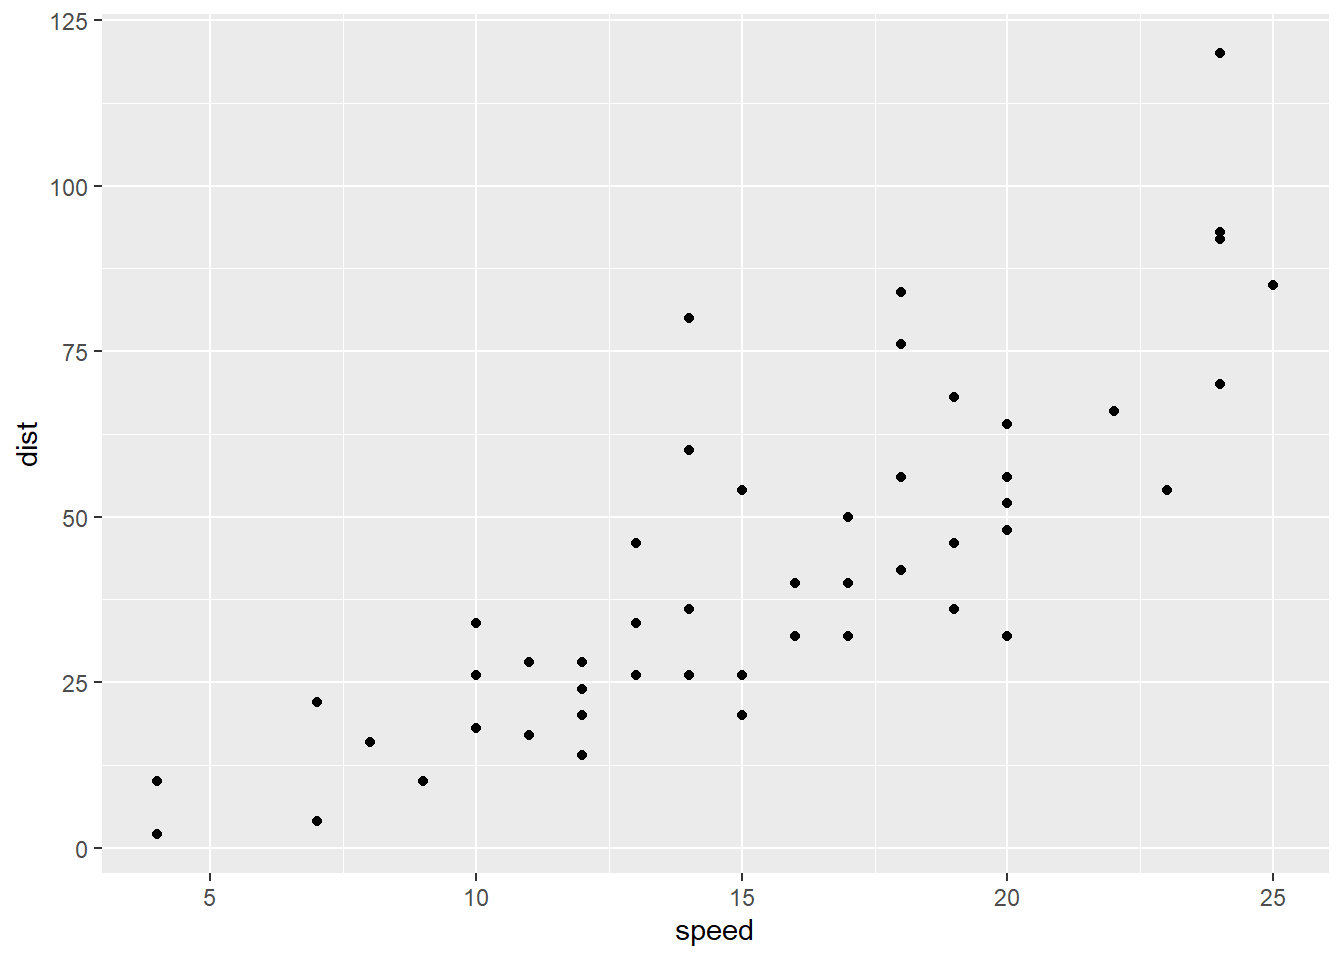
\includegraphics{_main_files/figure-latex/cars-plot-1.pdf}
\caption{\label{fig:cars-plot}A ggplot of car stuff}
\end{figure}

Under the hood, plots are included in your document in the same way as images - when you build the book or knit a chapter, the plot is automatically generated from your code, saved as an image, then included into the output document.

\hypertarget{including-tables}{%
\subsection{Including tables}\label{including-tables}}

Tables are usually included with the \texttt{kable} function from the \texttt{knitr} package.

Table \ref{tab:cars-table} shows the first rows of that cars data - read in your own data, then use this approach to automatically generate tables.

\begin{Shaded}
\begin{Highlighting}[]
\NormalTok{cars }\OperatorTok\StringTok{ }
\StringTok{  }\KeywordTok{head}\NormalTok{() }\OperatorTok\StringTok{ }
\StringTok{  }\NormalTok{knitr}\OperatorTok{::}\KeywordTok{kable}\NormalTok{(}\DataTypeTok{caption =} \StringTok{"A knitr kable table"}\NormalTok{)}
\end{Highlighting}
\end{Shaded}

\begin{table}

\caption{\label{tab:cars-table}A knitr kable table}
\centering
\begin{tabular}[t]{r|r}
\hline
speed & dist\\
\hline
4 & 2\\
\hline
4 & 10\\
\hline
7 & 4\\
\hline
7 & 22\\
\hline
8 & 16\\
\hline
9 & 10\\
\hline
\end{tabular}
\end{table}

\begin{itemize}
\tightlist
\item
  Gotcha: when using \href{https://www.rdocumentation.org/packages/knitr/versions/1.21/topics/kable}{\texttt{kable}}, captions are set inside the \texttt{kable} function
\item
  The \texttt{kable} package is often used with the \href{https://cran.r-project.org/web/packages/kableExtra/vignettes/awesome_table_in_html.html}{\texttt{kableExtra}} package
\end{itemize}

\hypertarget{a-note-on-content-positioning}{%
\subsection{A note on content positioning}\label{a-note-on-content-positioning}}

One thing that may be annoying is the way \emph{R Markdown} handles ``floats'' like tables and figures.

In your PDF output, LaTeX will try to find the best place to put your object based on the text around it and until you're really, truly done writing you should just leave it where it lies.

When the time comes for you to make final tweaks to content positioning, read the relevant \href{https://bookdown.org/yihui/rmarkdown/}{R Markdown documentation} to see if there are easy ways to do what you want.

If you have very specific needs, you might have to read up on LaTeX (\url{https://en.wikibooks.org/wiki/LaTeX/Floats,_Figures_and_Captions}) for your PDF output and/or on how to style HTML documents with CSS for your gitbook output.

\hypertarget{inline-code-1}{%
\section{Inline code}\label{inline-code-1}}

`Inline code' simply means inclusion of code inside text.

The syntax for doing this is \texttt{\textasciigrave{}r\ R\_CODE\textasciigrave{}}

For example, \texttt{\textasciigrave{}r\ 4\ +\ 4\textasciigrave{}} would output 8 in your text.

You will usually use this in parts of your thesis where you report results - read in data or results in a code chunk, store things you want to report in a variable, then insert the value of that variable in your text.

For example, we might assign the number of rows in the \texttt{cars} dataset to a variable:

\begin{Shaded}
\begin{Highlighting}[]
\NormalTok{num_car_observations <-}\StringTok{ }\KeywordTok{nrow}\NormalTok{(cars)}
\end{Highlighting}
\end{Shaded}

We might then write:\\
``In the \texttt{cars} dataset, we have \texttt{\textasciigrave{}r\ num\_car\_observations\textasciigrave{}} observations.''

Which would output:\\
``In the \texttt{cars} dataset, we have 50 observations.''

\hypertarget{referring-to-results-computed-in-other-languages-than-r}{%
\subsection{Referring to results computed in other languages than R}\label{referring-to-results-computed-in-other-languages-than-r}}

I've commented the below section out, to avoid compilation errors from the \texttt{reticulate} package being unable to find a python installation (after I installed MacOS Catalina, \texttt{reticulate} was unable to select a python version on my system, and I had to set it manually with \texttt{use\_python}).

If you need to use other langauges, have a look at the content I commented out by the end of the \textbf{02-rmd-basics-code.Rmd} file, which gives an example of using Python in your R Markdown file.

\hypertarget{cites-and-refs}{%
\chapter{Citations and cross-references}\label{cites-and-refs}}

\chaptermark{Cites and cross-refs}

\hypertarget{citations}{%
\section{Citations}\label{citations}}

The usual way to include citations in an \emph{R Markdown} document is to put references in a plain text file with the extension \textbf{.bib}, in \textbf{BibTex} format.\footnote{The bibliography can be in other formats as well, including EndNote (\textbf{.enl}) and RIS (\textbf{.ris}), see \href{https://rmarkdown.rstudio.com/authoring_bibliographies_and_citations.html}{rmarkdown.rstudio.com/authoring\_bibliographies\_and\_citations}.}
Then reference the path to this file in \textbf{index.Rmd}'s YAML header with \texttt{bibliography:\ example.bib}.

Most reference managers can create a .bib file with you references automatically.
However, the \textbf{by far} best reference manager to use with \emph{R Markdown} is \href{https://www.zotero.org}{Zotero} with the \href{https://retorque.re/zotero-better-bibtex/}{Better BibTex plug-in}, because the \texttt{citr} plugin for RStudio (see below) can read references directly from your Zotero library!

Here is an example of an entry in a \textbf{.bib} file:

\begin{Shaded}
\begin{Highlighting}[]
\VariableTok{@article}\NormalTok{\{}\OtherTok{Shea2014}\NormalTok{,}
  \DataTypeTok{author}\NormalTok{ =        \{Shea, Nicholas and Boldt, Annika\},}
  \DataTypeTok{journal}\NormalTok{ =       \{Trends in Cognitive Sciences\},}
  \DataTypeTok{pages}\NormalTok{ =         \{186--193\},}
  \DataTypeTok{title}\NormalTok{ =         \{\{Supra-personal cognitive control\}\},}
  \DataTypeTok{volume}\NormalTok{ =        \{18\},}
  \DataTypeTok{year}\NormalTok{ =          \{2014\},}
  \DataTypeTok{doi}\NormalTok{ =           \{10.1016/j.tics.2014.01.006\},}
\NormalTok{\}}
\end{Highlighting}
\end{Shaded}

In this entry highlighed section, `Shea2014' is the \textbf{citation identifier}.
To default way to cite an entry in your text is with this syntax: \texttt{{[}@citation-identifier{]}}.

So I might cite some things \autocite{Shea2014,Lottridge2012}.

\hypertarget{pdf-output}{%
\subsection{PDF output}\label{pdf-output}}

In PDF output, the bibliography is handled by the OxThesis LaTeX template.
If you set \texttt{bib-humanities:\ true} in \textbf{index.Rmd}, then in-text references will be formatted as author-year; otherwise references will be shown as numbers.

If you choose author-year formatting, a number of variations on the citation syntax are useful to know:

\begin{itemize}
\tightlist
\item
  Put author names outside the parenthesis

  \begin{itemize}
  \tightlist
  \item
    This: \texttt{@Shea2014\ says\ blah.}
  \item
    Becomes: \textcite{Shea2014} says blah.
  \end{itemize}
\item
  Include only the citation-year (in parenthesis)

  \begin{itemize}
  \tightlist
  \item
    This: \texttt{Shea\ et\ al.\ says\ blah\ {[}-@Shea2014{]}}
  \item
    Becomes: Shea et al.~says blah \autocite*{Shea2014}
  \end{itemize}
\item
  Add text and page or chapter references to the citation

  \begin{itemize}
  \tightlist
  \item
    This: \texttt{{[}see\ @Shea2014,\ pp.\ 33-35;\ also\ @Wu2016,\ ch.\ 1{]}}
  \item
    Becomes: Blah blah \autocites[see][pp.~33-35]{Shea2014}[also][ch.~1]{Wu2016}.
  \end{itemize}
\end{itemize}

\hypertarget{gitbook-output}{%
\subsection{Gitbook output}\label{gitbook-output}}

In gitbook output, citations are by default inserted in the Chicago author-date format.

To change the format, add \texttt{csl:\ some-other-style.csl} in \textbf{index.Rmd}'s YAML header.
You can browse through and download styles at \href{https://www.zotero.org/styles}{zotero.org/styles}.

\clearpage

\hypertarget{insert-references-easily-with-the-citr-add-in}{%
\subsection{\texorpdfstring{Insert references easily with the \texttt{citr} add-in}{Insert references easily with the citr add-in}}\label{insert-references-easily-with-the-citr-add-in}}

For an easy way to insert citations, try the \href{https://github.com/crsh/citr}{\texttt{citr}} RStudio add-in (Figure \ref{fig:citr}).
You can install this add-in by typing \texttt{install.packages("citr")} in the R Console.

\begin{figure}

{\centering \includegraphics[width=0.8\linewidth]{figures/citr} 

}

\caption{The `citr` add-in}\label{fig:citr}
\end{figure}

\hypertarget{cross-referencing}{%
\section{Cross-referencing}\label{cross-referencing}}

We can make cross-references to \textbf{sections} within our document, as well as to \textbf{figures} (images and plots) and \textbf{tables}.

The general cross-referencing syntax is \textbf{\texttt{\textbackslash{}@ref(label)}}

\hypertarget{section-references}{%
\subsection{Section references}\label{section-references}}

Headers are automatically assigned a reference label, which is the text in lower caps separated by dashes. For example, \texttt{\#\ My\ header} is automatically given the label \texttt{my-header}. So \texttt{\#\ My\ header} can be referenced with \texttt{\textbackslash{}@ref(my-section)}

Remember what we wrote in section \ref{citations}?

We can also use \textbf{hyperlink syntax} and add \# before the label, though this is only guaranteed to work properly in HTML output:

\begin{itemize}
\tightlist
\item
  So if we write \texttt{Remember\ what\ we\ wrote\ up\ in\ {[}the\ previous\ section{]}(\#citations)?}
\item
  It becomes Remember what we wrote up in \protect\hyperlink{citations}{the previous section}?
\end{itemize}

\hypertarget{creating-custom-labels}{%
\subsubsection{Creating custom labels}\label{creating-custom-labels}}

It is a very good idea to create \textbf{custom labels} for our sections. This is because the automatically assigned labels will change when we change the titles of the sections - to avoid this, we can create the labels ourselves and leave them untouched if we change the section titles.

We create custom labels by adding \texttt{\{\#label\}} after a header, e.g.~\texttt{\#\ My\ section\ \{\#my-label\}}.
See \protect\hyperlink{cites-and-refs}{our chapter title} for an example. That was section \ref{cites-and-refs}.

\hypertarget{figure-image-and-plot-references}{%
\subsection{Figure (image and plot) references}\label{figure-image-and-plot-references}}

\begin{itemize}
\tightlist
\item
  To refer to figures (i.e.~images and plots) use the syntax \texttt{\textbackslash{}@ref(fig:label)}
\item
  \textbf{GOTCHA}: Figures and tables must have captions if you wish to cross-reference them.
\end{itemize}

Let's add an image:

\begin{Shaded}
\begin{Highlighting}[]
\NormalTok{knitr}\OperatorTok{::}\KeywordTok{include_graphics}\NormalTok{(}\StringTok{"figures/captain.jpeg"}\NormalTok{)}
\end{Highlighting}
\end{Shaded}

\begin{figure}

{\centering \includegraphics[width=0.65\linewidth]{figures/captain} 

}

\caption{A marvel-lous meme}\label{fig:captain}
\end{figure}

We refer to this image with \texttt{\textbackslash{}@ref(fig:captain)}.
So Figure \ref{fig:captain} is \protect\hyperlink{fig:captain}{this image}.

And in Figure \ref{fig:cars-plot} we saw a \protect\hyperlink{fig:cars-plot}{cars plot}.

\hypertarget{table-references}{%
\subsection{Table references}\label{table-references}}

\begin{itemize}
\tightlist
\item
  To refer to tables use the syntax \texttt{\textbackslash{}@ref(tab:label)}
\end{itemize}

Let's include a table:

\begin{Shaded}
\begin{Highlighting}[]
\NormalTok{knitr}\OperatorTok{::}\KeywordTok{kable}\NormalTok{(cars[}\DecValTok{1}\OperatorTok{:}\DecValTok{5}\NormalTok{,],}
            \DataTypeTok{caption=}\StringTok{"Stopping cars"}\NormalTok{)}
\end{Highlighting}
\end{Shaded}

\begin{table}

\caption{\label{tab:cars-table2}Stopping cars}
\centering
\begin{tabular}[t]{r|r}
\hline
speed & dist\\
\hline
4 & 2\\
\hline
4 & 10\\
\hline
7 & 4\\
\hline
7 & 22\\
\hline
8 & 16\\
\hline
\end{tabular}
\end{table}

We refer to this table with \texttt{\textbackslash{}@ref(tab:cars-table2)}.
So Table \ref{tab:cars-table2} is \protect\hyperlink{tab:cars-table2}{this table}.

And in Table \ref{tab:cars-table} we saw more or less \protect\hyperlink{tab:cars-table}{the same cars table}.

\hypertarget{including-page-numbers}{%
\subsection{Including page numbers}\label{including-page-numbers}}

Finally, in the PDF output we might also want to include the page number of a reference, so that it's easy to find in physical printed output.
LaTeX has a command for this, which looks like this: \texttt{\textbackslash{}pageref\{fig/tab:label\}} (note: curly braces, not parentheses)

When we output to PDF, we can use raw LaTeX directly in our .Rmd files. So if we wanted to include the page of the cars plot we could write:

\begin{itemize}
\tightlist
\item
  This: \texttt{Figure\ \textbackslash{}@ref(fig:cars-plot)\ on\ page\ \textbackslash{}pageref(fig:cars-plot)}
\item
  Becomes: Figure \ref{fig:cars-plot} on page \pageref{fig:cars-plot}
\end{itemize}

\hypertarget{include-page-numbers-only-in-pdf-output}{%
\subsubsection{Include page numbers only in PDF output}\label{include-page-numbers-only-in-pdf-output}}

A problem here is that LaTeX commands don't display in HTML output, so in the gitbook output we'd see simply ``Figure \ref{fig:cars-plot} on page''.

One way to get around this is to use inline R code to insert the text, and use an \texttt{ifelse} statement to check the output format and then insert the appropriate text.

\begin{itemize}
\tightlist
\item
  So this: \texttt{\textasciigrave{}r\ ifelse(knitr::is\_latex\_output(),\ "Figure\ \textbackslash{}\textbackslash{}@ref(fig:cars-plot)\ on\ page\ \textbackslash{}\textbackslash{}pageref\{fig:cars-plot\}",\ "")\textasciigrave{}}
\item
  Inserts this (check this on both PDF and gitbook): Figure \ref{fig:cars-plot} on page \pageref{fig:cars-plot}
\end{itemize}

Note that we need to escape the backslash with another backslash here to get the correct output.

\hypertarget{customising-your-thesis-front-matter-n-stuff}{%
\section{Customising your thesis' front matter 'n stuff}\label{customising-your-thesis-front-matter-n-stuff}}

\hypertarget{shorten-captions-shown-in-the-list-of-figures-pdf}{%
\subsection{Shorten captions shown in the list of figures (PDF)}\label{shorten-captions-shown-in-the-list-of-figures-pdf}}

You might want your list of figures (which follows the table of contents) to have shorter (or just different) figure descriptions than the actual figure captions.

Do this using the chunk option \texttt{fig.scap} (`short caption'), for example \texttt{\{r\ captain-image,\ fig.cap="A\ very\ long\ and\ descriptive\ (and\ potentially\ boring)\ caption\ that\ doesn\textquotesingle{}t\ fit\ in\ the\ list\ of\ figures,\ but\ helps\ the\ reader\ understand\ what\ the\ figure\ communicates.",\ fig.scap="A\ concise\ description\ for\ the\ list\ of\ figures"}

\hypertarget{shorten-captions-shown-in-the-list-of-tables-pdf}{%
\subsection{Shorten captions shown in the list of tables (PDF)}\label{shorten-captions-shown-in-the-list-of-tables-pdf}}

You might want your list of tables (which follows the list of figures in your thesis front matter) to have shorter (or just different) table descriptions than the actual table captions.

If you are using \texttt{knitr::kable} to generate a table, you can do this with the argument \texttt{caption.short}, e.g.:

\begin{Shaded}
\begin{Highlighting}[]
\NormalTok{knitr}\OperatorTok{::}\KeywordTok{kable}\NormalTok{(mtcars,}
              \DataTypeTok{caption =} \StringTok{"A very long and descriptive (and potentially}
\StringTok{              boring) caption that doesn't fit in the list of figures,}
\StringTok{              but helps the reader understand what the figure }
\StringTok{              communicates."}\NormalTok{,}
              \DataTypeTok{caption.short =} \StringTok{"A concise description for the list of tables"}\NormalTok{)}
\end{Highlighting}
\end{Shaded}

\hypertarget{shorting-the-running-header-pdf}{%
\subsection{Shorting the running header (PDF)}\label{shorting-the-running-header-pdf}}

You might want a chapter's running header (i.e.~the header showing the title of the current chapter at the top of page) to be shorter (or just different) to the actual chapter title.

Do this by adding the latex command \texttt{\textbackslash{}chaptermark\{My\ shorter\ version\}} after your chapter title.

For example, this chapter's running header is simply `Cites and cross-refs', because it begins like this:

\begin{Shaded}
\begin{Highlighting}[]
\FunctionTok{# Citations and cross-references \{#cites-and-refs\}}
\NormalTok{\textbackslash{}chaptermark\{Cites and cross-refs\}}
\end{Highlighting}
\end{Shaded}

\hypertarget{final-notes-on-the-huthesis-template-and-on-collaboration}{%
\chapter{Final Notes on The HUThesis template and on collaboration}\label{final-notes-on-the-huthesis-template-and-on-collaboration}}

\hypertarget{beginning-chapters-with-quotes}{%
\section{Beginning chapters with quotes}\label{beginning-chapters-with-quotes}}

The HUThesis LaTeX template lets you inject some wittiness into your thesis by including a block of type \texttt{savequote} at the beginning of chapters.
To do this, use the syntax \texttt{\textasciigrave{}\textasciigrave{}\textasciigrave{}\{block\ type=\textquotesingle{}savequote\textquotesingle{}\}}.\footnote{For more on custom block types, see the relevant section in \href{https://bookdown.org/yihui/bookdown/custom-blocks.html}{\emph{Authoring Books with R Markdown}}.}

Add the reference for the quote with the chunk option \texttt{quote\_author="my\ author\ name"}.
You will also want to add the chunk option \texttt{include=knitr::is\_latex\_output()} so that quotes are only included in PDF output.

It's not possible to use markdown syntax inside chunk options, so if you want to e.g.~italicise a book name in the reference use a \href{https://bookdown.org/yihui/bookdown/markdown-extensions-by-bookdown.html\#text-references}{`text reference'}: Create a named piece of text with `(ref:label-name) My text', then point to this in the chunk option with \texttt{quote\_author=\textquotesingle{}(ref:label-name)\textquotesingle{}}.

\hypertarget{highlighting-corrections}{%
\section{Highlighting corrections}\label{highlighting-corrections}}

For when it comes time to do corrections, you may want to highlight changes made when you submit a post-viva, corrected copy to your examiners so they can quickly verify you've completed the task.
You can do so like this:

\hypertarget{short-inline-corrections}{%
\subsection{Short, inline corrections}\label{short-inline-corrections}}

Highlight \textbf{short, inline corrections} by doing \texttt{{[}like\ this{]}\{.correction\}} --- the text between the square brackets will then \colorbox[HTML]{CCCCFF}{be highlighted in blue} in the output.

\hypertarget{blocks-of-added-or-changed-material}{%
\subsection{Blocks of added or changed material}\label{blocks-of-added-or-changed-material}}

Highlight entire \textbf{blocks of added or changed material} by putting them in a block of type \texttt{correction}, using the syntax \texttt{\textasciigrave{}\textasciigrave{}\textasciigrave{}\{block\ type=\textquotesingle{}correction\textquotesingle{}\}}.\footnote{In the \textbf{.tex} file for PDF output, this will put the content between \texttt{\textbackslash{}begin\{correction\}} and \texttt{\textbackslash{}end\{correction\}}; in gitbook output it will be put between \texttt{\textless{}div\ class="correction"\textgreater{}} and \texttt{\textless{}/div\textgreater{}}.}
Like so:

\begin{verbatim}
For larger chunks, like this paragraph or indeed entire figures, you can use the `correction` block type. This environment **highlights paragraph-sized and larger blocks** with the same blue colour.
\end{verbatim}

\hypertarget{stopping-corrections-from-being-highlighted-in-the-output}{%
\subsection{Stopping corrections from being highlighted in the output}\label{stopping-corrections-from-being-highlighted-in-the-output}}

For \textbf{PDF} output, go to \textbf{index.Rmd} and (i) set \texttt{corrections:\ false} under \texttt{params} in the YAML header (stops block of corrections from being highlighted), (ii) comment out \texttt{pandoc\_args:\ {[}"-\/-lua-filter=scripts\_and\_filters/correction\_filter.lua"{]}} (stops inline corrections from being highlighted).

For \textbf{gitbook} output, go to \textbf{style.css} and comment out the styling for \texttt{.correction}.

\hypertarget{diving-in-to-the-oxthesis-latex-template}{%
\section{Diving in to the OxThesis LaTeX template}\label{diving-in-to-the-oxthesis-latex-template}}

For LaTeX minded people, you can read through \textbf{templates/template.tex} to see which additional customisation options are available as well as \textbf{templates/ociamthesis.cls} which supplies the base class.
For example, \textbf{template.tex} provides an option for master's degree submissions, which changes identifying information to candidate number and includes a word count.
At the time of writing, you must set this directly in \textbf{template.tex} rather than from the YAML header in \textbf{index.Rmd}.

\hypertarget{collaborative-writing}{%
\section{Collaborative writing}\label{collaborative-writing}}

Best practices for collaboration and change tracking when using R Markdown are still an open question.
In the blog post \href{https://livefreeordichotomize.com/2018/09/14/one-year-to-dissertate/}{\textbf{One year to dissertate}} by Lucy D'Agostino, which I highly recommend, the author notes that she knits .Rmd files to a \texttt{word\_document}, then uses the \texttt{googledrive} R package to send this to Google Drive for comments / revisions from co-authors, then incorporates Google Drive suggestions \emph{by hand} into the .Rmd source files.
This is a bit clunky, and there are ongoing discussions among the \emph{R Markdown} developers about what the best way is to handle collaborative writing (see \href{https://github.com/rstudio/rmarkdown/issues/1463}{issue \#1463} on GitHub, where \href{http://criticmarkup.com}{CriticMarkup} is among the suggestions).

For now, this is an open question in the community of R Markdown users.
I often knit to a format that can easily be imported to Google Docs for comments, then go over suggested revisions and manually incorporate them back in to the .Rmd source files.
For articles, I sometimes upload a near-final draft to \href{https://www.overleaf.com/}{Overleaf}, then collaboratively make final edits to the \LaTeX~file there.
I suspect some great solution will be developed in the not-to-distant future, probably by the RStudio team.

\hypertarget{customisations-and-extensions}{%
\chapter{Customisations and extensions}\label{customisations-and-extensions}}

This chapter describes a number of possible customizations to the \texttt{oxforddown} thesis.

\hypertarget{embedding-pdf-documents-as-chapters}{%
\section{Embedding PDF documents as chapters}\label{embedding-pdf-documents-as-chapters}}

You may want to embed existing PDF documents into the thesis, for example if your department allows a `portfolio' style thesis and you need to include an existing typeset publication as a chapter.

In gitbook output, you can simply use \texttt{knitr::include\_graphics} and it should include a scrollable (and downloadable) PDF.
You will probably want to set the chunk options \texttt{out.width=\textquotesingle{}100\%\textquotesingle{}} and \texttt{out.height=\textquotesingle{}1000px\textquotesingle{}}:

\begin{Shaded}
\begin{Highlighting}[]
\NormalTok{knitr}\OperatorTok{::}\KeywordTok{include_graphics}\NormalTok{(}\StringTok{"figures/pdf_example/Lyngs2020_FB.pdf"}\NormalTok{)}
\end{Highlighting}
\end{Shaded}

In LaTeX output, however, this approach can cause odd behaviour.
Therefore, when you build your thesis to PDF, split the PDF into an alphanumerically sorted sequence of \textbf{single-page} PDF files (you can do this automatically with the package \texttt{pdftools}). You can then use the appropriate LaTeX command to insert them, as shown below (for brevity, in the \texttt{oxforddown} PDF sample content we're only including two pages)
\emph{Note that the chunk option \texttt{results=\textquotesingle{}asis\textquotesingle{}} must be set.}
You may also want to remove margins from the PDF files, which you can do with Adobe Acrobat (paid version) and likely other software.

\begin{Shaded}
\begin{Highlighting}[]
\CommentTok{# install.packages(pdftools)}
\CommentTok{# split PDF into pages stored in figures/pdf_example/split/}
\CommentTok{# pdftools::pdf_split("figures/pdf_example/Lyngs2020_FB.pdf",}
\CommentTok{# output = "figures/pdf_example/split/")}

\CommentTok{# grab the pages}
\NormalTok{pages <-}\StringTok{ }\KeywordTok{list.files}\NormalTok{(}\StringTok{"figures/pdf_example/split"}\NormalTok{, }\DataTypeTok{full.names =} \OtherTok{TRUE}\NormalTok{)}

\CommentTok{# set how wide you want the inserted PDFs to be:}
\CommentTok{# 1.0 is 100 per cent of the oxforddown PDF page width;}
\CommentTok{# you may want to make it a bit bigger}
\NormalTok{pdf_width <-}\StringTok{ }\FloatTok{1.2}

\CommentTok{# for each PDF page, insert it nicely and}
\CommentTok{# end with a page break}
\KeywordTok{cat}\NormalTok{(stringr}\OperatorTok{::}\KeywordTok{str_c}\NormalTok{(}\StringTok{"}\CharTok{\textbackslash{}\textbackslash{}}\StringTok{newpage }\CharTok{\textbackslash{}\textbackslash{}}\StringTok{begin\{center\}}
\StringTok{    }\CharTok{\textbackslash{}\textbackslash{}}\StringTok{makebox[}\CharTok{\textbackslash{}\textbackslash{}}\StringTok{linewidth][c]\{}\CharTok{\textbackslash{}\textbackslash{}}\StringTok{includegraphics[width="}\NormalTok{, pdf_width,}
    \StringTok{"}\CharTok{\textbackslash{}\textbackslash{}}\StringTok{linewidth]\{"}\NormalTok{, pages, }\StringTok{"\}\} }\CharTok{\textbackslash{}\textbackslash{}}\StringTok{end\{center\}"}\NormalTok{))}
\end{Highlighting}
\end{Shaded}

\newpage \begin{center} \makebox[\linewidth][c]{\includegraphics[width=1.2\linewidth]{figures/pdf_example/split/_000000000000001.pdf}} \end{center} \newpage \begin{center} \makebox[\linewidth][c]{\includegraphics[width=1.2\linewidth]{figures/pdf_example/split/_000000000000011.pdf}} \end{center}

\hypertarget{customizing-referencing}{%
\section{Customizing referencing}\label{customizing-referencing}}

\hypertarget{using-a-.csl-file-with-pandoc-instead-of-biblatex}{%
\subsection{Using a .csl file with pandoc instead of biblatex}\label{using-a-.csl-file-with-pandoc-instead-of-biblatex}}

The \texttt{oxforddown} package uses biblatex in latex for referencing.
It is also possible to use pandoc for referencing by providing a .csl file in the YAML header of \textbf{index.Rmd} (likely requiring commenting out the biblatex code in \textbf{templates/template.tex}).
This may be helpful for those who have a .csl file describing the referencing format for a particular journal.
However, note that this approach does not support chapter bibliographies (see Section \ref{biblatex-custom}).

\begin{Shaded}
\begin{Highlighting}[]
\FunctionTok{csl:}\AttributeTok{ ecology.csl}
\end{Highlighting}
\end{Shaded}

\hypertarget{biblatex-custom}{%
\subsection{Customizing biblatex and adding chapter bibliographies}\label{biblatex-custom}}

This section provides one example of customizing biblatex. Much of this code was combined from searches on Stack Exchange and other sources (e.g.~\href{https://tex.stackexchange.com/questions/10682/suppress-in-biblatex}{here}).

In \textbf{templates/template.tex}, one can replace the existing biblatex calls with the following to achieve referencing that looks like this:

(Charmantier and Gienapp 2014)

Charmantier, A. and P. Gienapp (2014). Climate change and timing of avian breeding and migration: evolutionary versus plastic changes. Evolutionary Applications 7(1):15--28. doi: 10.1111/eva.12126.

\begin{Shaded}
\begin{Highlighting}[]
\BuiltInTok{\textbackslash{}usepackage}\NormalTok{[backend=biber,}
\NormalTok{    bibencoding=utf8,}
\NormalTok{    refsection=chapter, }\CommentTok{% referencing by chapter}
\NormalTok{    style=authoryear, }
\NormalTok{    firstinits=true,}
\NormalTok{    isbn=false,}
\NormalTok{    doi=true,}
\NormalTok{    url=false,}
\NormalTok{    eprint=false,}
\NormalTok{    related=false,}
\NormalTok{    dashed=false,}
\NormalTok{    clearlang=true,}
\NormalTok{    maxcitenames=2,}
\NormalTok{    mincitenames=1,}
\NormalTok{    maxbibnames=10,}
\NormalTok{    abbreviate=false,}
\NormalTok{    minbibnames=3,}
\NormalTok{    uniquelist=minyear,}
\NormalTok{    sortcites=true,}
\NormalTok{    date=year}
\NormalTok{]\{}\ExtensionTok{biblatex}\NormalTok{\}}
\FunctionTok{\textbackslash{}AtEveryBibitem}\NormalTok{\{}\CommentTok
  \FunctionTok{\textbackslash{}clearfield}\NormalTok{\{note\}}
\NormalTok{\}}

\FunctionTok{\textbackslash{}DeclareFieldFormat}\NormalTok{\{titlecase\}\{}\FunctionTok{\textbackslash{}MakeTitleCase}\NormalTok{\{#1\}\}}

\FunctionTok{\textbackslash{}newrobustcmd}\NormalTok{\{}\FunctionTok{\textbackslash{}MakeTitleCase}\NormalTok{\}[1]\{}\CommentTok
    \FunctionTok{\textbackslash{}OR\textbackslash{}ifcurrentfield}\NormalTok{\{maintitle\}}\FunctionTok{\textbackslash{}OR\textbackslash{}ifcurrentfield}\NormalTok{\{mainsubtitle\}}\CommentTok
    \FunctionTok{\textbackslash{}OR\textbackslash{}ifcurrentfield}\NormalTok{\{issuetitle\}}\FunctionTok{\textbackslash{}OR\textbackslash{}ifcurrentfield}\NormalTok{\{issuesubtitle\}}\CommentTok
    \FunctionTok{\textbackslash{}OR\textbackslash{}ifentrytype}\NormalTok{\{booklet\}}\FunctionTok{\textbackslash{}OR\textbackslash{}ifentrytype}\NormalTok{\{suppbook\}}\CommentTok
    \FunctionTok{\textbackslash{}OR\textbackslash{}ifentrytype}\NormalTok{\{suppcollection\}}\FunctionTok{\textbackslash{}OR\textbackslash{}ifentrytype}\NormalTok{\{manual\}}\CommentTok
    \FunctionTok{\textbackslash{}OR\textbackslash{}ifentrytype}\NormalTok{\{proceedings\}}\FunctionTok{\textbackslash{}OR\textbackslash{}ifentrytype}\NormalTok{\{mvproceedings\}}\CommentTok
    \FunctionTok{\textbackslash{}OR\textbackslash{}ifentrytype}\NormalTok{\{report\}}\FunctionTok{\textbackslash{}OR\textbackslash{}ifentrytype}\NormalTok{\{thesis\}\}}
\NormalTok{    \{#1\}}
\NormalTok{    \{}\FunctionTok{\textbackslash{}MakeSentenceCase}\NormalTok{\{#1\}\}\}}
    
\CommentTok{% \textbackslash{}renewbibmacro\{in:\}\{\}}
\CommentTok{% suppress "in" for articles}
\CommentTok
  \FunctionTok{\textbackslash{}ifentrytype}\NormalTok{\{article\}\{\}\{}\FunctionTok{\textbackslash{}printtext}\NormalTok{\{}\FunctionTok{\textbackslash{}bibstring}\NormalTok{\{in\}}\FunctionTok{\textbackslash{}intitlepunct}\NormalTok{\}\}\}}
\CommentTok{%-- no "quotes" around titles of chapters/article titles}
\FunctionTok{\textbackslash{}DeclareFieldFormat}\NormalTok{[article, inbook, incollection, inproceedings, misc, thesis, unpublished]}
\NormalTok{\{title\}\{#1\}}
\CommentTok{%-- no punctuation after volume}
\FunctionTok{\textbackslash{}DeclareFieldFormat}\NormalTok{[article]}
\NormalTok{\{volume\}\{\{#1\}\}}
\CommentTok{%-- puts number/issue between brackets}
\FunctionTok{\textbackslash{}DeclareFieldFormat}\NormalTok{[article, inbook, incollection, inproceedings, misc, thesis, unpublished]}
\NormalTok{\{number\}\{}\FunctionTok{\textbackslash{}mkbibparens}\NormalTok{\{#1\}\} }
\CommentTok{%-- and then for articles directly the pages w/o any "pages" or "pp." }
\FunctionTok{\textbackslash{}DeclareFieldFormat}\NormalTok{[article]}
\NormalTok{\{pages\}\{#1\}}
\CommentTok{%-- for some types replace "pages" by "p."}
\FunctionTok{\textbackslash{}DeclareFieldFormat}\NormalTok{[inproceedings, incollection, inbook]}
\NormalTok{\{pages\}\{p. #1\}}
\CommentTok
  \FunctionTok{\textbackslash{}printfield}\NormalTok{\{number\}}\CommentTok{%}
  \FunctionTok{\textbackslash{}printunit}\NormalTok{\{}\FunctionTok{\textbackslash{}addcolon}\NormalTok{\}}
\NormalTok{\}}
\end{Highlighting}
\end{Shaded}

If you would like chapter bibliographies, in addition insert the following code at the end of each chapter, and comment out the entire REFERENCES section at the end of template.tex.

\begin{Shaded}
\begin{Highlighting}[]
\FunctionTok{\textbackslash{}printbibliography}\NormalTok{[segment=}\FunctionTok{\textbackslash{}therefsection}\NormalTok{,heading=subbibliography]}
\end{Highlighting}
\end{Shaded}

\hypertarget{customizing-the-page-headers-and-footers}{%
\section{Customizing the page headers and footers}\label{customizing-the-page-headers-and-footers}}

The following code, when it replaces the existing correpsonding code block in \textbf{ociamthesis.cls}, puts chapter number and title centered in the header and page number in the footer, centered.
This may be desirable particularly when inserting PDF chapters, as the margins of the PDF may not exactly align with the left and right margins of the page, demarcated by the existing header and footer text.
In the following code block, the original code is commented out where replaced.

\begin{Shaded}
\begin{Highlighting}[]
\BuiltInTok{\textbackslash{}usepackage}\NormalTok{\{}\ExtensionTok{fancyhdr}\NormalTok{\}}
\FunctionTok{\textbackslash{}setlength}\NormalTok{\{}\FunctionTok{\textbackslash{}headheight}\NormalTok{\}\{15pt\}}
\FunctionTok{\textbackslash{}fancyhf}\NormalTok{\{\} }\CommentTok{% clear the header and footers}
\FunctionTok{\textbackslash{}pagestyle}\NormalTok{\{fancy\}}
\FunctionTok{\textbackslash{}renewcommand}\NormalTok{\{}\ExtensionTok{\textbackslash{}chaptermark}\NormalTok{\}[1]\{}\FunctionTok{\textbackslash{}markboth}\NormalTok{\{}\FunctionTok{\textbackslash{}thechapter}\NormalTok{. #1\}\{}\FunctionTok{\textbackslash{}thechapter}\NormalTok{. #1\}\}}
\CommentTok{% \textbackslash{}renewcommand\{\textbackslash{}chaptermark\}[1]\{\textbackslash{}markboth\{\textbackslash{}thechapter. #1\}\{\}\}}
\FunctionTok{\textbackslash{}renewcommand}\NormalTok{\{}\ExtensionTok{\textbackslash{}sectionmark}\NormalTok{\}[1]\{}\FunctionTok{\textbackslash{}markright}\NormalTok{\{}\FunctionTok{\textbackslash{}thesection}\NormalTok{. #1\}\}}
\FunctionTok{\textbackslash{}renewcommand}\NormalTok{\{}\ExtensionTok{\textbackslash{}headrulewidth}\NormalTok{\}\{0pt\}}
\FunctionTok{\textbackslash{}fancyhead}\NormalTok{[CO]\{}\FunctionTok{\textbackslash{}emph}\NormalTok{\{}\FunctionTok{\textbackslash{}leftmark}\NormalTok{\}\}}
\FunctionTok{\textbackslash{}fancyhead}\NormalTok{[CE]\{}\FunctionTok{\textbackslash{}emph}\NormalTok{\{}\FunctionTok{\textbackslash{}rightmark}\NormalTok{\}\}}
\CommentTok{% \textbackslash{}fancyhead[LO,RE]\{\}}
\CommentTok{% \textbackslash{}fancyhead[LE,RO]\{\}}
\FunctionTok{\textbackslash{}fancyfoot}\NormalTok{[CO,CE]\{}\FunctionTok{\textbackslash{}emph}\NormalTok{\{}\FunctionTok{\textbackslash{}thepage}\NormalTok{\}\}}

\FunctionTok{\textbackslash{}fancypagestyle}\NormalTok{\{plain\}\{}\FunctionTok{\textbackslash{}fancyhf}\NormalTok{\{\}}\FunctionTok{\textbackslash{}fancyfoot}\NormalTok{[C]\{}\FunctionTok{\textbackslash{}emph}\NormalTok{\{}\FunctionTok{\textbackslash{}thepage}\NormalTok{\}\}\}}

\CommentTok{% JEM fix header on cleared pages for openright}
\FunctionTok{\textbackslash{}def}\NormalTok{\textbackslash{}cleardoublepage\{\textbackslash{}clearpage\textbackslash{}if@twoside \textbackslash{}ifodd\textbackslash{}c@page\textbackslash{}else}
\NormalTok{   \textbackslash{}hbox\{\}}
   \CommentTok{% \textbackslash{}fancyhead[RE,LO]\{\}}
\NormalTok{   \textbackslash{}fancyhead[CE,CO]\{\}}
\NormalTok{   \textbackslash{}newpage}
\NormalTok{   \textbackslash{}if@twocolumn\textbackslash{}hbox\{\}\textbackslash{}newpage}
\NormalTok{   \textbackslash{}fi}
   \CommentTok{% \textbackslash{}fancyhead[LO]\{\textbackslash{}emph\{\textbackslash{}leftmark\}\} }
   \CommentTok{% \textbackslash{}fancyhead[RE]\{\textbackslash{}emph\{\textbackslash{}rightmark\}\} }
\NormalTok{   \textbackslash{}fancyhead[CO]\{\textbackslash{}emph\{\textbackslash{}leftmark\}\} }
\NormalTok{   \textbackslash{}fancyhead[CE]\{\textbackslash{}emph\{\textbackslash{}rightmark\}\} }
\NormalTok{   \textbackslash{}fi\textbackslash{}fi\}}
\end{Highlighting}
\end{Shaded}

\hypertarget{conclusion}{%
\chapter{Conclusion}\label{conclusion}}

If we don't want Conclusion to have a chapter number next to it, we can add the \texttt{\{-\}} attribute.
\autocite{von_goethe_wilhelm_1829}

\textbf{More info}

And here's some other random info: the first paragraph after a chapter title or section head \emph{shouldn't be} indented, because indents are to tell the reader that you're starting a new paragraph. Since that's obvious after a chapter or section title, proper typesetting doesn't add an indent there.

%%%%% REFERENCES

% JEM: Quote for the top of references (just like a chapter quote if you're using them).  Comment to skip.
% \begin{savequote}[8cm]
% The first kind of intellectual and artistic personality belongs to the hedgehogs, the second to the foxes \dots
%   \qauthor{--- Sir Isaiah Berlin \cite{berlin_hedgehog_2013}}
% \end{savequote}

\setlength{\baselineskip}{0pt} % JEM: Single-space References

{\renewcommand*\MakeUppercase[1]{#1}%
\printbibliography[heading=bibintoc,title={\bibtitle}]}

\hypertarget{appendix-appendix}{%
\appendix}


\hypertarget{the-first-appendix}{%
\chapter{The First Appendix}\label{the-first-appendix}}

This first appendix includes an R chunk that was hidden in the document (using \texttt{echo\ =\ FALSE}) to help with readibility:

\textbf{In 02-rmd-basics-code.Rmd}

\begin{Shaded}
\begin{Highlighting}[]
\KeywordTok{library}\NormalTok{(tidyverse)}
\NormalTok{knitr}\OperatorTok{::}\KeywordTok{include_graphics}\NormalTok{(}\StringTok{"figures/chunk-parts.png"}\NormalTok{)}
\end{Highlighting}
\end{Shaded}

\textbf{And here's another one from the same chapter, i.e.~Chapter \ref{code}:}

\hypertarget{the-second-appendix-for-fun}{%
\chapter{The Second Appendix, for Fun}\label{the-second-appendix-for-fun}}

\end{document}
